\documentclass{standalone}
\usepackage{tikz}
\usetikzlibrary{patterns, positioning}
\usepackage[sfdefault]{ClearSans} %% option 'sfdefault' activates Clear Sans as the default text font
\usepackage[T1]{fontenc}

\begin{document}
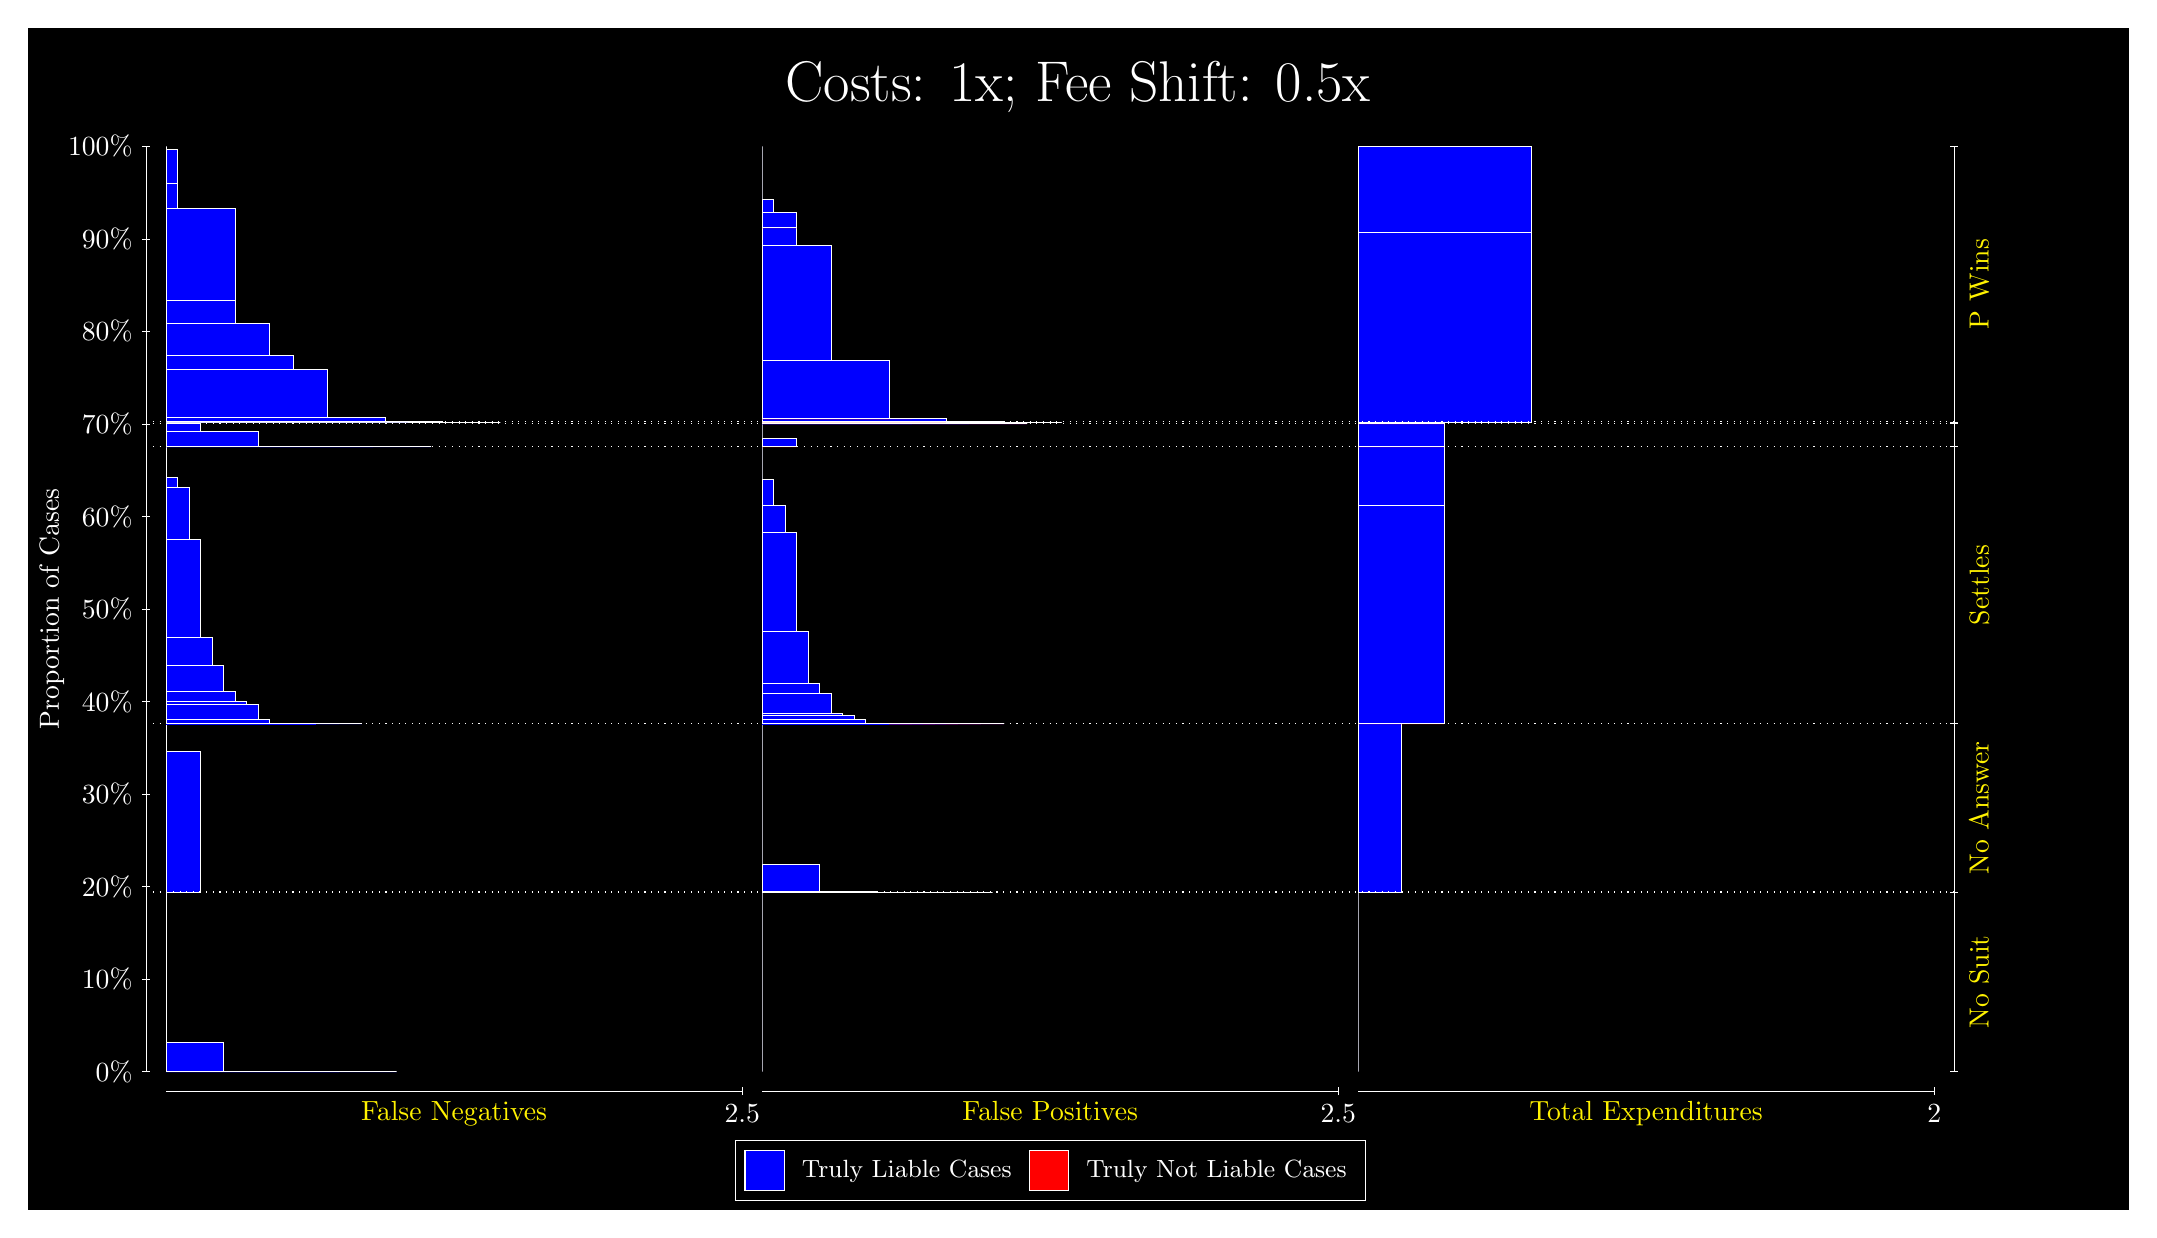
\begin{tikzpicture}
\draw[fill=black] (0,0) rectangle (26.667,15);
\draw[text=white] (0,13.5) rectangle (26.667,15) node[midway] {\huge Costs: 1x; Fee Shift: 0.5x};
\draw[white, very thin] (1.5,1.75) -- (1.5,13.5);
\node[rotate=90, text=white, anchor=center] at (0.3, 7.625) {Proportion of Cases};
\draw[white, very thin] (1.45,1.75) -- (1.55,1.75);
\node[text=white, anchor=east] at (1.45, 1.75) {0\%};
\draw[white, very thin] (1.45,2.925) -- (1.55,2.925);
\node[text=white, anchor=east] at (1.45, 2.925) {10\%};
\draw[white, very thin] (1.45,4.1) -- (1.55,4.1);
\node[text=white, anchor=east] at (1.45, 4.1) {20\%};
\draw[white, very thin] (1.45,5.275) -- (1.55,5.275);
\node[text=white, anchor=east] at (1.45, 5.275) {30\%};
\draw[white, very thin] (1.45,6.45) -- (1.55,6.45);
\node[text=white, anchor=east] at (1.45, 6.45) {40\%};
\draw[white, very thin] (1.45,7.625) -- (1.55,7.625);
\node[text=white, anchor=east] at (1.45, 7.625) {50\%};
\draw[white, very thin] (1.45,8.8) -- (1.55,8.8);
\node[text=white, anchor=east] at (1.45, 8.8) {60\%};
\draw[white, very thin] (1.45,9.975) -- (1.55,9.975);
\node[text=white, anchor=east] at (1.45, 9.975) {70\%};
\draw[white, very thin] (1.45,11.15) -- (1.55,11.15);
\node[text=white, anchor=east] at (1.45, 11.15) {80\%};
\draw[white, very thin] (1.45,12.325) -- (1.55,12.325);
\node[text=white, anchor=east] at (1.45, 12.325) {90\%};
\draw[white, very thin] (1.45,13.5) -- (1.55,13.5);
\node[text=white, anchor=east] at (1.45, 13.5) {100\%};

\draw[white, very thin] (24.457,1.75) -- (24.457,13.5);
\draw[white, very thin] (24.407,1.75) -- (24.507,1.75);
\node[anchor=west] at (24.407, 1.75) {};
\draw[white, very thin] (24.407,4.0302) -- (24.507,4.0302);
\node[anchor=west] at (24.407, 4.0302) {};
\draw[white, very thin] (24.407,6.1691) -- (24.507,6.1691);
\node[anchor=west] at (24.407, 6.1691) {};
\draw[white, very thin] (24.407,9.6873) -- (24.507,9.6873);
\node[anchor=west] at (24.407, 9.6873) {};
\draw[white, very thin] (24.407,9.9772) -- (24.507,9.9772);
\node[anchor=west] at (24.407, 9.9772) {};
\draw[white, very thin] (24.407,10.001) -- (24.507,10.001);
\node[anchor=west] at (24.407, 10.001) {};
\draw[white, very thin] (24.407,13.5) -- (24.507,13.5);
\node[anchor=west] at (24.407, 13.5) {};

\draw[white, very thin, fill=blue] (1.75,1.75) rectangle (4.6775,1.75);
\draw[white, very thin, fill=blue] (1.75,1.75) rectangle (3.9457,1.75);
\draw[white, very thin, fill=blue] (1.75,1.75) rectangle (3.2138,1.7532);
\draw[white, very thin, fill=blue] (1.75,1.7532) rectangle (2.4819,2.1234);
\draw[white, very thin, fill=red] (1.75,2.1234) rectangle (1.75,2.1234);
\draw[white, very thin, fill=blue] (1.75,2.1234) rectangle (1.75,4.0302);
\draw[white, very thin, fill=blue] (1.75,4.0302) rectangle (2.1891,5.8188);
\draw[white, very thin, fill=red] (1.75,5.8188) rectangle (1.75,5.8188);
\draw[white, very thin, fill=blue] (1.75,5.8188) rectangle (1.75,6.1691);
\draw[white, very thin, fill=blue] (1.75,6.1691) rectangle (4.2384,6.1691);
\draw[white, very thin, fill=blue] (1.75,6.1691) rectangle (3.9457,6.1691);
\draw[white, very thin, fill=blue] (1.75,6.1691) rectangle (3.6529,6.1694);
\draw[white, very thin, fill=blue] (1.75,6.1694) rectangle (3.5065,6.1695);
\draw[white, very thin, fill=blue] (1.75,6.1695) rectangle (3.3602,6.1698);
\draw[white, very thin, fill=blue] (1.75,6.1698) rectangle (3.2138,6.1714);
\draw[white, very thin, fill=blue] (1.75,6.1714) rectangle (3.0674,6.2233);
\draw[white, very thin, fill=blue] (1.75,6.2233) rectangle (2.921,6.4097);
\draw[white, very thin, fill=blue] (1.75,6.4097) rectangle (2.7746,6.4573);
\draw[white, very thin, fill=blue] (1.75,6.4573) rectangle (2.6283,6.5843);
\draw[white, very thin, fill=blue] (1.75,6.5843) rectangle (2.4819,6.9111);
\draw[white, very thin, fill=blue] (1.75,6.9111) rectangle (2.3355,7.2604);
\draw[white, very thin, fill=blue] (1.75,7.2604) rectangle (2.1891,8.511);
\draw[white, very thin, fill=blue] (1.75,8.511) rectangle (2.0428,9.1699);
\draw[white, very thin, fill=blue] (1.75,9.1699) rectangle (2.0428,9.1748);
\draw[white, very thin, fill=blue] (1.75,9.1748) rectangle (1.8964,9.301);
\draw[white, very thin, fill=red] (1.75,9.301) rectangle (1.75,9.301);
\draw[white, very thin, fill=blue] (1.75,9.301) rectangle (1.75,9.6873);
\draw[white, very thin, fill=blue] (1.75,9.6873) rectangle (5.1167,9.6873);
\draw[white, very thin, fill=blue] (1.75,9.6873) rectangle (4.3848,9.6873);
\draw[white, very thin, fill=blue] (1.75,9.6873) rectangle (3.6529,9.6935);
\draw[white, very thin, fill=blue] (1.75,9.6935) rectangle (2.921,9.8751);
\draw[white, very thin, fill=blue] (1.75,9.8751) rectangle (2.1891,9.9772);
\draw[white, very thin, fill=red] (1.75,9.9772) rectangle (1.75,9.9772);
\draw[white, very thin, fill=blue] (1.75,9.9772) rectangle (2.1891,9.9978);
\draw[white, very thin, fill=red] (1.75,9.9978) rectangle (1.75,9.9978);
\draw[white, very thin, fill=blue] (1.75,9.9978) rectangle (1.75,10.001);
\draw[white, very thin, fill=blue] (1.75,10.001) rectangle (5.9949,10.001);
\draw[white, very thin, fill=blue] (1.75,10.001) rectangle (5.2631,10.002);
\draw[white, very thin, fill=blue] (1.75,10.002) rectangle (4.8239,10.002);
\draw[white, very thin, fill=blue] (1.75,10.002) rectangle (4.5312,10.059);
\draw[white, very thin, fill=blue] (1.75,10.059) rectangle (4.092,10.059);
\draw[white, very thin, fill=blue] (1.75,10.059) rectangle (3.7993,10.674);
\draw[white, very thin, fill=blue] (1.75,10.674) rectangle (3.3602,10.841);
\draw[white, very thin, fill=blue] (1.75,10.841) rectangle (3.0674,11.258);
\draw[white, very thin, fill=blue] (1.75,11.258) rectangle (2.6283,11.543);
\draw[white, very thin, fill=blue] (1.75,11.543) rectangle (2.6283,12.719);
\draw[white, very thin, fill=blue] (1.75,12.719) rectangle (2.3355,12.719);
\draw[white, very thin, fill=blue] (1.75,12.719) rectangle (1.8964,13.031);
\draw[white, very thin, fill=blue] (1.75,13.031) rectangle (1.8964,13.458);
\draw[white, very thin, fill=red] (1.75,13.458) rectangle (1.75,13.458);
\draw[white, very thin, fill=blue] (1.75,13.458) rectangle (1.75,13.5);
\draw[white, very thin, fill=red] (9.3189,1.75) rectangle (9.3189,1.75);
\draw[white, very thin, fill=blue] (9.3189,1.75) rectangle (9.3189,4.0302);
\draw[white, very thin, fill=red] (9.3189,4.0302) rectangle (12.246,4.0302);
\draw[white, very thin, fill=blue] (9.3189,4.0302) rectangle (12.246,4.0302);
\draw[white, very thin, fill=blue] (9.3189,4.0302) rectangle (11.515,4.0302);
\draw[white, very thin, fill=blue] (9.3189,4.0302) rectangle (10.783,4.0332);
\draw[white, very thin, fill=blue] (9.3189,4.0332) rectangle (10.051,4.3804);
\draw[white, very thin, fill=blue] (9.3189,4.3804) rectangle (9.3189,6.1691);
\draw[white, very thin, fill=red] (9.3189,6.1691) rectangle (12.393,6.1691);
\draw[white, very thin, fill=blue] (9.3189,6.1691) rectangle (12.393,6.1691);
\draw[white, very thin, fill=red] (9.3189,6.1691) rectangle (12.1,6.1691);
\draw[white, very thin, fill=blue] (9.3189,6.1691) rectangle (12.1,6.1691);
\draw[white, very thin, fill=red] (9.3189,6.1691) rectangle (11.807,6.1691);
\draw[white, very thin, fill=blue] (9.3189,6.1691) rectangle (11.807,6.1691);
\draw[white, very thin, fill=blue] (9.3189,6.1691) rectangle (11.661,6.1691);
\draw[white, very thin, fill=red] (9.3189,6.1691) rectangle (11.515,6.1691);
\draw[white, very thin, fill=blue] (9.3189,6.1691) rectangle (11.515,6.1691);
\draw[white, very thin, fill=blue] (9.3189,6.1691) rectangle (11.368,6.1691);
\draw[white, very thin, fill=red] (9.3189,6.1691) rectangle (11.222,6.1691);
\draw[white, very thin, fill=blue] (9.3189,6.1691) rectangle (11.222,6.1691);
\draw[white, very thin, fill=blue] (9.3189,6.1691) rectangle (11.075,6.1691);
\draw[white, very thin, fill=red] (9.3189,6.1691) rectangle (10.929,6.1691);
\draw[white, very thin, fill=blue] (9.3189,6.1691) rectangle (10.929,6.1698);
\draw[white, very thin, fill=blue] (9.3189,6.1698) rectangle (10.783,6.17);
\draw[white, very thin, fill=blue] (9.3189,6.17) rectangle (10.636,6.17);
\draw[white, very thin, fill=red] (9.3189,6.17) rectangle (10.636,6.17);
\draw[white, very thin, fill=blue] (9.3189,6.17) rectangle (10.636,6.2193);
\draw[white, very thin, fill=blue] (9.3189,6.2193) rectangle (10.49,6.279);
\draw[white, very thin, fill=blue] (9.3189,6.279) rectangle (10.344,6.2965);
\draw[white, very thin, fill=blue] (9.3189,6.2965) rectangle (10.197,6.5553);
\draw[white, very thin, fill=blue] (9.3189,6.5553) rectangle (10.051,6.6815);
\draw[white, very thin, fill=blue] (9.3189,6.6815) rectangle (9.9044,6.6864);
\draw[white, very thin, fill=blue] (9.3189,6.6864) rectangle (9.9044,7.3454);
\draw[white, very thin, fill=blue] (9.3189,7.3454) rectangle (9.758,8.5959);
\draw[white, very thin, fill=blue] (9.3189,8.5959) rectangle (9.6116,8.9452);
\draw[white, very thin, fill=blue] (9.3189,8.9452) rectangle (9.4652,9.272);
\draw[white, very thin, fill=blue] (9.3189,9.272) rectangle (9.3189,9.6873);
\draw[white, very thin, fill=red] (9.3189,9.6873) rectangle (9.758,9.6873);
\draw[white, very thin, fill=blue] (9.3189,9.6873) rectangle (9.758,9.7894);
\draw[white, very thin, fill=blue] (9.3189,9.7894) rectangle (9.3189,9.9772);
\draw[white, very thin, fill=red] (9.3189,9.9772) rectangle (12.686,9.9772);
\draw[white, very thin, fill=blue] (9.3189,9.9772) rectangle (12.686,9.9772);
\draw[white, very thin, fill=blue] (9.3189,9.9772) rectangle (11.954,9.9772);
\draw[white, very thin, fill=blue] (9.3189,9.9772) rectangle (11.222,9.9773);
\draw[white, very thin, fill=blue] (9.3189,9.9773) rectangle (10.49,9.9807);
\draw[white, very thin, fill=blue] (9.3189,9.9807) rectangle (9.758,10.001);
\draw[white, very thin, fill=red] (9.3189,10.001) rectangle (13.125,10.001);
\draw[white, very thin, fill=blue] (9.3189,10.001) rectangle (13.125,10.001);
\draw[white, very thin, fill=red] (9.3189,10.001) rectangle (12.393,10.001);
\draw[white, very thin, fill=blue] (9.3189,10.001) rectangle (12.393,10.002);
\draw[white, very thin, fill=red] (9.3189,10.002) rectangle (11.661,10.002);
\draw[white, very thin, fill=blue] (9.3189,10.002) rectangle (11.661,10.043);
\draw[white, very thin, fill=red] (9.3189,10.043) rectangle (11.222,10.043);
\draw[white, very thin, fill=blue] (9.3189,10.043) rectangle (11.222,10.043);
\draw[white, very thin, fill=red] (9.3189,10.043) rectangle (10.929,10.043);
\draw[white, very thin, fill=blue] (9.3189,10.043) rectangle (10.929,10.782);
\draw[white, very thin, fill=red] (9.3189,10.782) rectangle (10.49,10.782);
\draw[white, very thin, fill=blue] (9.3189,10.782) rectangle (10.49,10.783);
\draw[white, very thin, fill=blue] (9.3189,10.783) rectangle (10.197,12.243);
\draw[white, very thin, fill=blue] (9.3189,12.243) rectangle (9.758,12.467);
\draw[white, very thin, fill=red] (9.3189,12.467) rectangle (9.758,12.467);
\draw[white, very thin, fill=blue] (9.3189,12.467) rectangle (9.758,12.66);
\draw[white, very thin, fill=blue] (9.3189,12.66) rectangle (9.4652,12.827);
\draw[white, very thin, fill=blue] (9.3189,12.827) rectangle (9.3189,13.5);
\draw[white, very thin, fill=red] (16.888,1.75) rectangle (16.888,1.75);
\draw[white, very thin, fill=blue] (16.888,1.75) rectangle (16.888,4.0302);
\draw[white, very thin, fill=red] (16.888,4.0302) rectangle (17.437,4.0302);
\draw[white, very thin, fill=blue] (16.888,4.0302) rectangle (17.437,6.1691);
\draw[white, very thin, fill=red] (16.888,6.1691) rectangle (17.986,6.1691);
\draw[white, very thin, fill=blue] (16.888,6.1691) rectangle (17.986,8.9441);
\draw[white, very thin, fill=red] (16.888,8.9441) rectangle (17.986,8.9441);
\draw[white, very thin, fill=blue] (16.888,8.9441) rectangle (17.986,9.6873);
\draw[white, very thin, fill=red] (16.888,9.6873) rectangle (17.986,9.6873);
\draw[white, very thin, fill=blue] (16.888,9.6873) rectangle (17.986,9.9772);
\draw[white, very thin, fill=red] (16.888,9.9772) rectangle (17.986,9.9772);
\draw[white, very thin, fill=blue] (16.888,9.9772) rectangle (17.986,10.001);
\draw[white, very thin, fill=red] (16.888,10.001) rectangle (19.083,10.001);
\draw[white, very thin, fill=blue] (16.888,10.001) rectangle (19.083,12.41);
\draw[white, very thin, fill=red] (16.888,12.41) rectangle (19.083,12.41);
\draw[white, very thin, fill=blue] (16.888,12.41) rectangle (19.083,13.5);
\draw[white, dotted] (1.5,4.0302) -- (24.457,4.0302);
\draw[white, dotted] (1.5,6.1691) -- (24.457,6.1691);
\draw[white, dotted] (1.5,9.6873) -- (24.457,9.6873);
\draw[white, dotted] (1.5,9.9772) -- (24.457,9.9772);
\draw[white, dotted] (1.5,10.001) -- (24.457,10.001);
\draw[white, very thin] (1.75,1.5) -- (9.0689,1.5);
\node[text=yellow, anchor=north] at (5.4094, 1.5) {False Negatives};
\draw[white, very thin] (9.0689,1.45) -- (9.0689,1.55);
\node[text=white, anchor=north] at (9.0689, 1.45) {2.5};

\draw[white, very thin] (9.3189,1.5) -- (16.638,1.5);
\node[text=yellow, anchor=north] at (12.978, 1.5) {False Positives};
\draw[white, very thin] (16.638,1.45) -- (16.638,1.55);
\node[text=white, anchor=north] at (16.638, 1.45) {2.5};

\draw[white, very thin] (16.888,1.5) -- (24.207,1.5);
\node[text=yellow, anchor=north] at (20.547, 1.5) {Total Expenditures};
\draw[white, very thin] (24.207,1.45) -- (24.207,1.55);
\node[text=white, anchor=north] at (24.207, 1.45) {2};

\node[text=yellow, centered, rotate=90] at (24.777, 2.8901) {No Suit};
\node[text=yellow, centered, rotate=90] at (24.777, 5.0996) {No Answer};
\node[text=yellow, centered, rotate=90] at (24.777, 7.9282) {Settles};


\node[text=yellow, centered, rotate=90] at (24.777, 11.751) {P Wins};

\draw (12.978300999999998,1.5) node[draw=none] (baseCoordinate) {};
\begin{scope}[align=center]
        \matrix[scale=0.5, draw=white, below=0.5cm of baseCoordinate, nodes={draw}, column sep=0.1cm]{
            \node[rectangle, draw, minimum width=0.5cm, minimum height=0.5cm, fill=blue] {}; &
            \node[draw=none, font=\small, text=white] (B) {Truly Liable Cases}; &
            \node[rectangle, draw, minimum width=0.5cm, minimum height=0.5cm, fill=red] {}; &
            \node[draw=none, font=\small, text=white] (B) {Truly Not Liable Cases}; \\
            };
\end{scope}

\end{tikzpicture}
\end{document}